\documentclass{beamer}
%
% Choose how your presentation looks.
%
% For more themes, color themes and font themes, see:
% http://deic.uab.es/~iblanes/beamer_gallery/index_by_theme.html
%
\mode<presentation>
{
  \usetheme{Madrid}      % or try Darmstadt, Madrid, Warsaw, ...
  \usecolortheme{beaver} % or try albatross, beaver, crane, ...
  \usefonttheme{serif}  % or try serif, structurebold, ...
  \setbeamertemplate{navigation symbols}{}
  \setbeamertemplate{caption}[numbered]
} 

\usepackage[english]{babel}

\usepackage[utf8x]{inputenc}
\usepackage{xcolor}
\usepackage{listings}
\usepackage{textpos}

\lstset
{
    language=[LaTeX]TeX,
    breaklines=true,
    basicstyle=\tt\scriptsize,
    %commentstyle=\color{green}
    keywordstyle=\color{blue},
    %stringstyle=\color{black}
    identifierstyle=\color{magenta},
}

\renewcommand{\rmdefault}{phv} % Arial
\renewcommand{\sfdefault}{phv} % Arial

\setbeamertemplate{frametitle}[default][center]

\addtobeamertemplate{frametitle}{}{%
\begin{textblock*}{100mm}(.88\textwidth,-.87cm)

\includegraphics[height=0.8cm,width=1.3cm]{ffhslogo}
\end{textblock*}}


\addtobeamertemplate{frametitle}{}{%
\begin{textblock*}{100mm}(-.02\textwidth,-.9cm)

\includegraphics[height=1.5cm,width=1.5cm]{chip}
\end{textblock*}}


\title[Energie in der Informatik]{Struktur der Thesis}
\author{Samuel Riolo}
\institute{FFHS}
\date{23. April 2016}


\begin{document}

\begin{frame}
  \titlepage
\end{frame}

% Uncomment these lines for an automatically generated outline.
\begin{frame}{Outline}
\frametitle{Inhaltsverzeichnis}
    \tableofcontents[]
\end{frame}

\section{Struktur Einleitung} 
\begin{frame}
\frametitle{Struktur} 
\begin{itemize}
\item Titelseite                                      (1)
\item Abstract De/En                                  (1)
\item Abkürzungen                                     (1)
\item Inhaltsverzeichnis                              (1)

\item Einleitung                                      (5)
 \begin{itemize}
 \item Einführung
 \item Fragestellung
 \item Resultate
 \item Vorgehen     
 \end{itemize}
\end{itemize}

\end{frame}


\section{Struktur Hauptteil}
\begin{frame}
\frametitle{Struktur} 
\begin{itemize}
\item Energiepolitik 2050                             (7)
\begin{itemize}
 \item Stromnachfrage 2010 - 2050
 \item Strom als Rückgrat des zukünftigen Energiesystems
 \item Spezifische Stromgestehungskosten
 \item Entwicklung der IT-Infrastruktur
 \item Erneuerbare Energien
\end{itemize}
\end{itemize}

\end{frame}




\begin{frame}
\frametitle{Struktur} 
\begin{itemize}
\item Aufbau des Experiments (12)
 \begin{itemize}
 \item Ziel des Experiments / Warum diese Methode
 \item Beschreibung der Hardware
 \item Funktionsweise eines CPU
 \item Software Interrupts unter Linux
 \item Aufbau der Software für die Messung
 \item Automatisation der Messung 
 \end{itemize}
 \item Resultate (3)
 \begin{itemize}
 \item Darstellung + Unterschiede zwischen einzelnen Befehlsätzen
 \item Verbesserungsvorschläge
 \end{itemize}
\end{itemize}
\end{frame}

\section{Struktur Abschluss} 
\begin{frame}
\frametitle{Struktur} 
\begin{itemize}
\item Fazit (2)
\begin{itemize}
  \item Diskussion
  \item Vergleich mit ähnliche Papers (z.B. Energiemessung durch thermische Kamera)
  \item Das Resultat in Sätze gefasst
\end{itemize}
\item Quellen (2)

\item Anhang
\begin{itemize}
\item Code
\item Messresultate 
\end{itemize}

\end{itemize}
\end{frame}



\section{Zwischenstand}
\begin{frame}
\frametitle {Zwischenstand}
\begin{itemize}
 \item Experiment aufgebaut
 \item Einige Versuche konnten bereits gemacht werden
\end{itemize}
\end{frame}

\section{Zu erledigen}
\begin{frame}
\frametitle{Zu erledigen}
\begin{itemize}
 \item Methode verfeinern
 \item Messungen definieren
 \item Messungen durchführen
 \item Viel schreiben...
\end{itemize}

\end{frame}


\section{Demo (Optional je nach verfügbarer Zeit)} 
\begin{frame}
\Huge Demo

\begin{figure}
  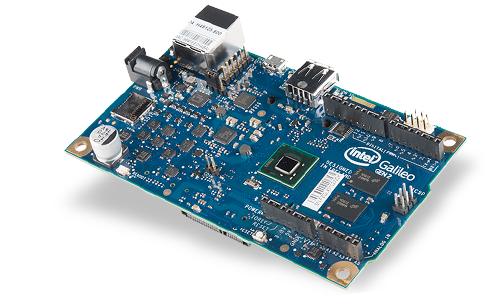
\includegraphics[width=200px,height=120px]{iot_galileo.png}
\end{figure}	

\end{frame}



 
\begin{frame}
\frametitle{Interrupts}
\begin{figure}
  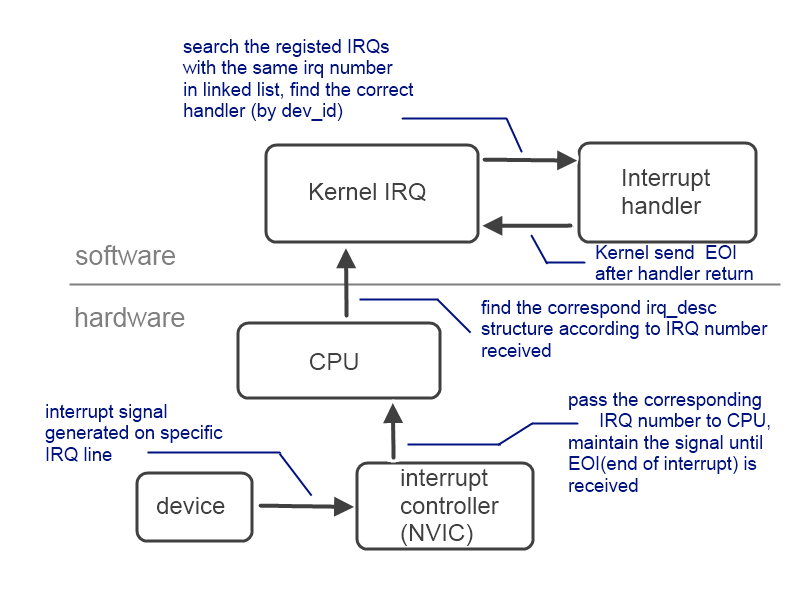
\includegraphics[width=280px,height=200px]{interrupt_view.png}
     \caption{hackpad-attachments.imgix.net}
\end{figure}	
\end{frame}


\begin{frame}
\frametitle{Interrupts}
\begin{figure}
  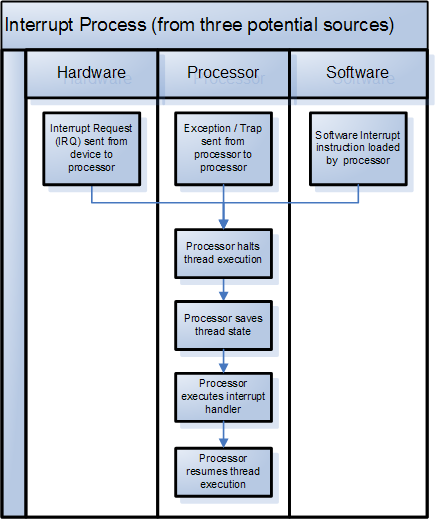
\includegraphics[width=185px,height=200px]{Interrupt_Process.PNG}
   \caption{wikipedia.org}
\end{figure}	

\end{frame}


\begin{frame}[fragile]
\frametitle{C} 

\lstset{language=C,
                basicstyle=\ttfamily\small,
                keywordstyle=\color{blue}\ttfamily,
                stringstyle=\color{red}\ttfamily,
                commentstyle=\color{green}\ttfamily,
                morecomment=[l][\color{magenta}]{\#}
}
\begin{lstlisting}
int benchmark_show_addl_32(struct seq_file* m, void* v)
{
    unsigned long long start_jif = get_jiffies_64();
    unsigned long long exec_jif;

    benchmark_addl_32();

    exec_jif = get_jiffies_64() - start_jif;
    seq_printf(m, "%llu\n", (unsigned long long)exec_jif);
    return 0;
}

\end{lstlisting}

\end{frame}





\begin{frame}[fragile]
\frametitle{Assembler} 


\lstdefinelanguage
   [x64]{Assembler}     % add a "x64" dialect of Assembler
   [x86masm]{Assembler} % based on the "x86masm" dialect
   % with these extra keywords:
   {morekeywords={CDQE,CQO,CMPSQ,CMPXCHG16B,JRCXZ,LODSQ,MOVSXD, %
                  POPFQ,PUSHFQ,SCASQ,STOSQ,IRETQ,RDTSCP,SWAPGS, %
                  rax,rdx,rcx,rbx,rsi,rdi,rsp,rbp, %
                  r8,r8d,r8w,r8b,r9,r9d,r9w,r9b}} % etc.

\lstset{language=[x64]Assembler}

\begin{lstlisting}
.globl benchmark_addl_32
.type benchmark_addl_32, @function

benchmark_addl_32:
  push %ecx
  movl $100000000, %ecx
  movl $0xFFFFFFFF, %eax
  movl $0xFFFFFFFF, %ebx
loop_benchmark_addl_32:
  addl %ebx, %eax
  movl $0xFFFFFFFF, %ebx
  loop loop_benchmark_addl_32
  pop %ecx
  ret
\end{lstlisting}
\end{frame}




\begin{frame}[fragile]
\lstdefinelanguage{Ini}
{
    basicstyle=\ttfamily\small,
    columns=fullflexible,
    morecomment=[s][\color{blue}\bfseries]{[}{]},
    morecomment=[l]{\#},
    morecomment=[l]{;},
    commentstyle=\color{gray}\ttfamily,
    morekeywords={},
    otherkeywords={=,:},
    keywordstyle={\color{green}\bfseries}
}

\lstset{language=Ini}
\frametitle{.ini Konfigurationsdatei} 

\begin{lstlisting}
[addl_32]
desc=2**32 + 2**32
pre=
  movl $0xFFFFFFFF, %eax
  movl $0xFFFFFFFF, %ebx
bench=
  addl %ebx, %eax
  movl $0xFFFFFFFF, %ebx
\end{lstlisting}
\end{frame}




\end{document}

